\providecommand*{\lstnumberautorefname}{line}
\subsection{Matrix Multiplication Example}
To demonstrate and highlight the potential saving that duplicating just
the control flow shadow can achieve we will use the classic example of
matrix multiplication, as seen in \hyperref[lst:MMM]{Listing \ref{lst:MMM}}.

\lstset{language=C}
\begin{lstlisting}[basicstyle=\ttfamily\footnotesize, frame=single, label={lst:MMM}, captionpos=b, caption={Matrix Multiplication Example},numbers=right,escapeinside={@}{@}]
void MMM(float A[5][5],float B[5][5],float C[5][5])
{ int i=0, j=0, k=0;
  for(i=0, i<5, i++){
    for(j=0, j<5; j++){
      C[i][j] = 0;
      for(k=0, k<5; k++){
        @\label{lst:MMM_2}@C[i][j] += A[i][k]*B[k][j]; }
    }
  }
}
\end{lstlisting}

The HLS generated circuit for this function can be divided into two main subsystems, the datapath, and the control FSM.
Within the datapath are all the functional units required to perform the computation, which in our example will contain:
integer comparators and incrementers for calculating the loop conditionals; and floating point adders and multipliers
for computing line \autoref{lst:MMM_2} of Listing \ref{lst:MMM}.
As the control FSM contains logic used for scheduling which operation is performed on a functional unit in the datapath,
when that operation is performed, and how data is moved between functional units.

If our matrix multiplication circuit was left unprotected to operate in the presence of soft errors then upsets within
the floating point addition and multiplication circuitry could potentially cause the data in the output
matrix to be incorrect.
This is however arguably less catastrophic than errors in the integer functional units since all integer operations
are involved in control flow decisions within the program.
Such errors could cause the calculation of rows and columns of the output matrix \lstinline$C$ to be skipped, or even
worse, cause the circuit to enter an infinite loop and never terminate.

Let's say in this example the engineer developing our system has determined that errors within
the output are tolerable or can be detected through statistical means at a later point.
Despite this however they are required to ensure that the circuit takes the correct number of cycles to
execute and always terminates.
One of the more obvious initial things that our engineer might try is full circuit replication, duplicating both the
control FSM an the datapath but will quickly discover how expensive this is in terms of power and resources.
Since errors in the output can be tolerated, our engineer might try and duplicate just the control FSM however
many of the state transitions within the control FSM are dependant on the outputs of results in the datapath.
Eventually  they realise that in this case by removing the expensive floating point units from the datapath
they can protect all the control decisions of the input program while reducing the amount of resources required
to do so.

Performing a manual inspection of the code and removing elements that have no influence on the program control flow
may be feasible in the case of Matrix Multiplication, however as the complexity of the input program increases
the engineering effort required in both analysing the input source and generating circuits with an identical control FSM is
significant.
StitchUp fully automates this process through using a static analysis technique, known as program slicing, to extract
and duplicate any instructions that may influence control.


\begin{figure}[!t]
\centering
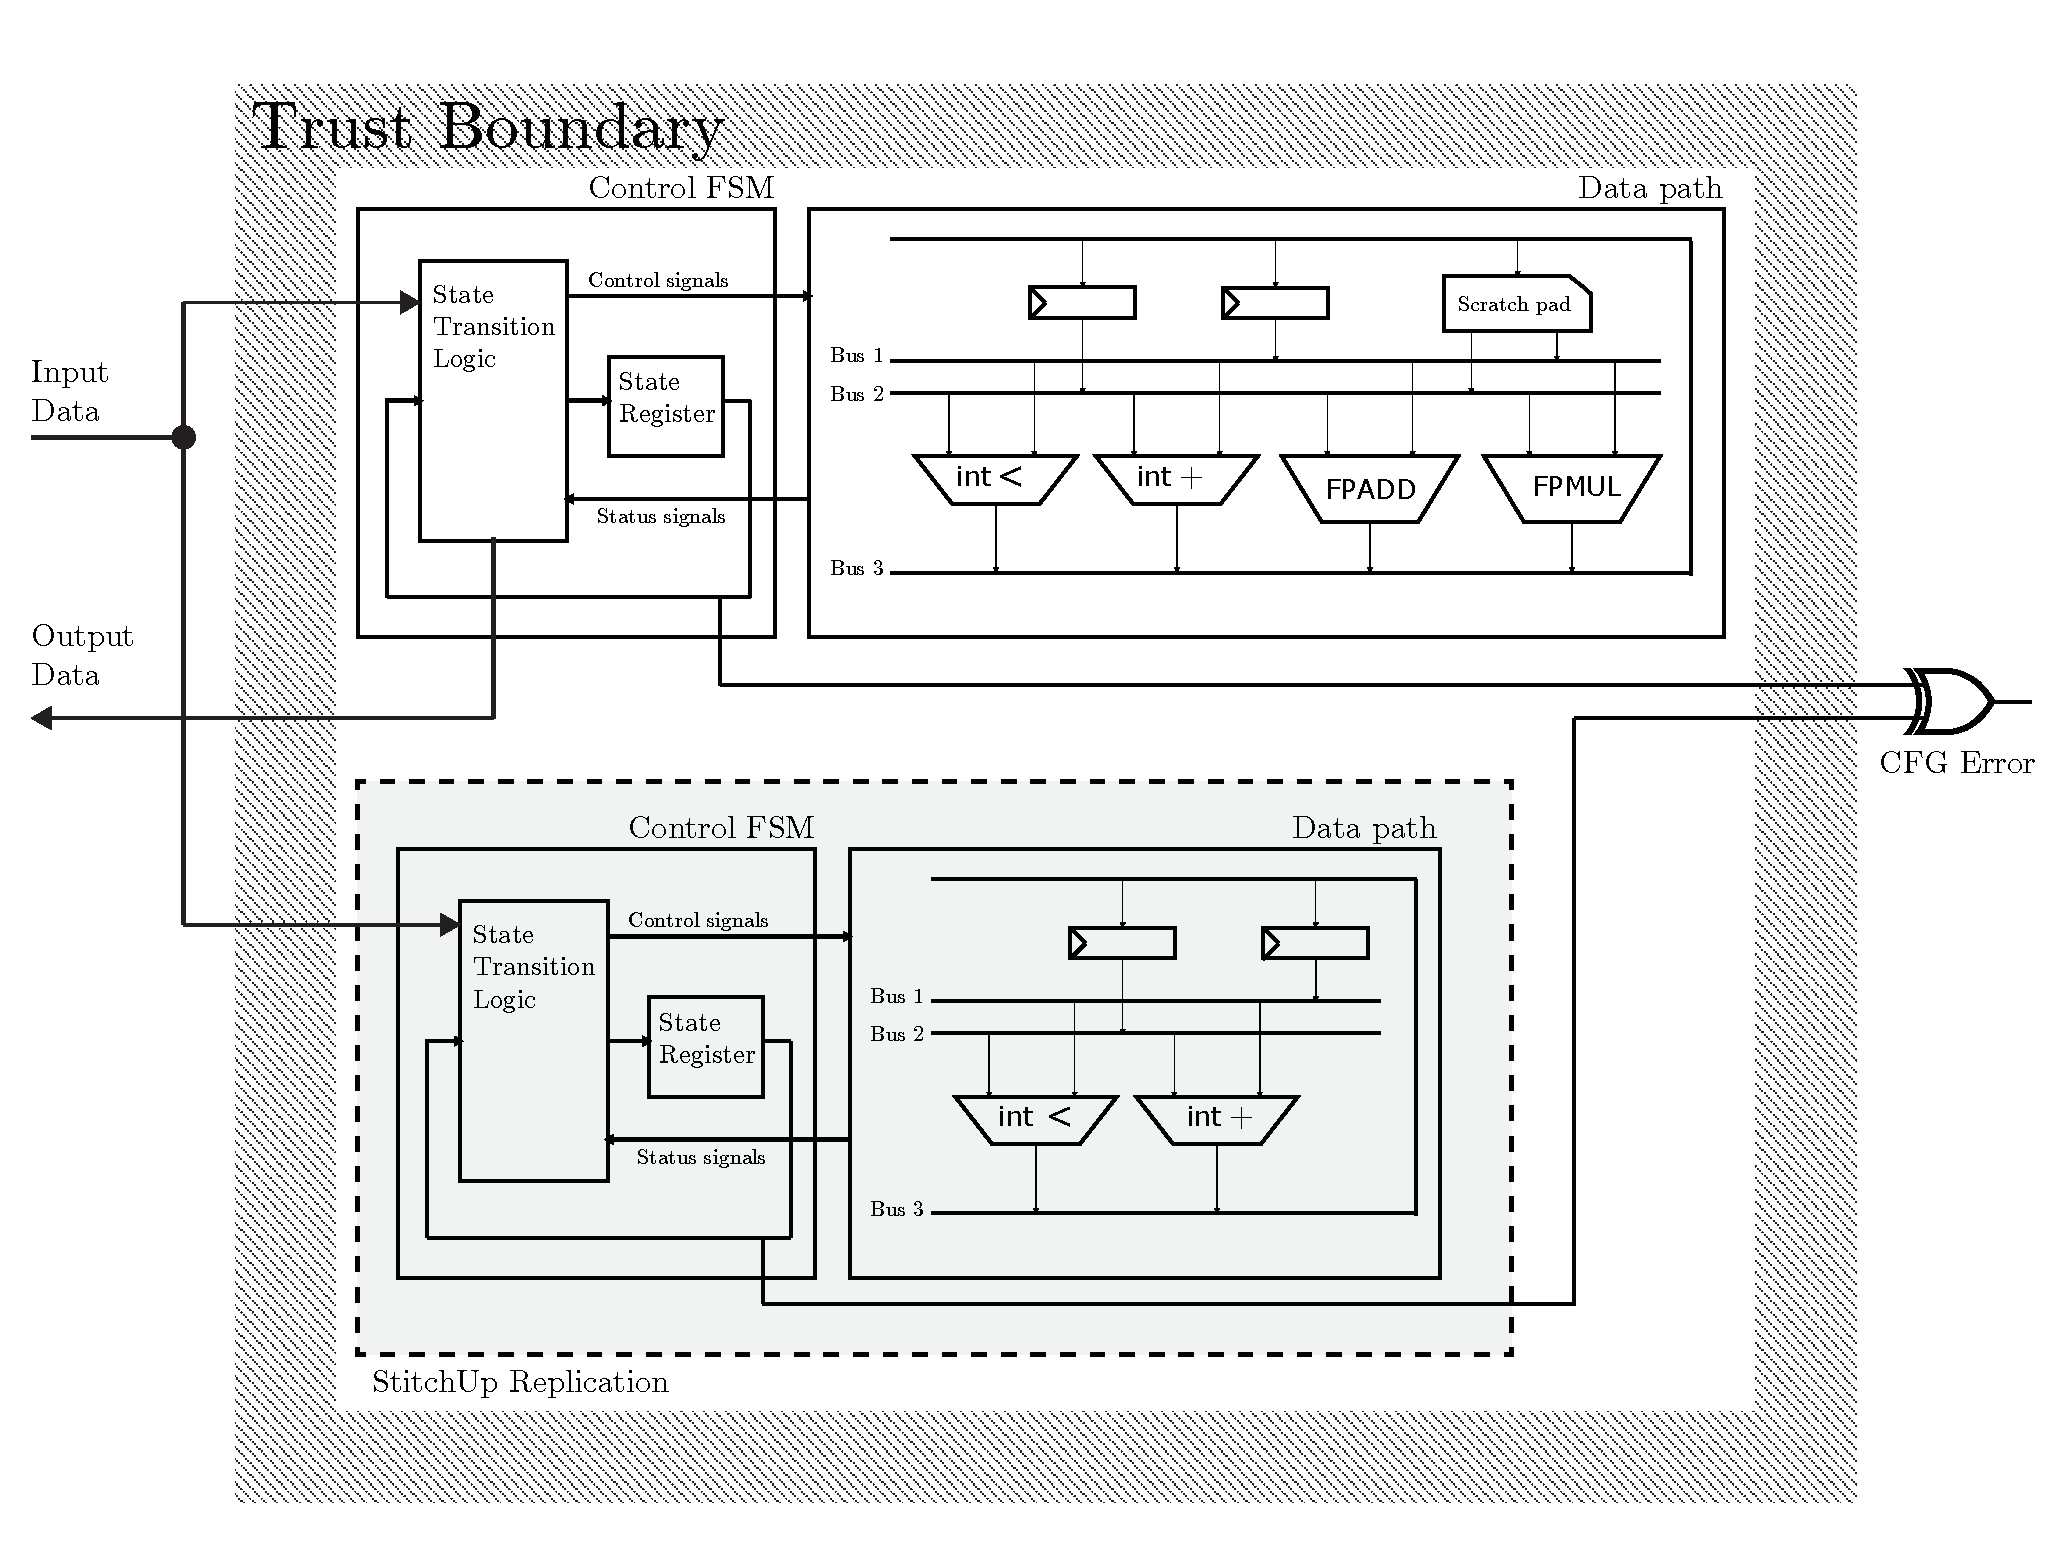
\includegraphics[width=3.5in]{./imgs/HLSArch.pdf}
\caption{StitchUp Replication for the Matrix Multiplication example, with Trust Boundary}
\label{fig:HLSArch}
\end{figure}

\subsection{Threat Model}
What is the threat model?
Use some Set notation to make what is being protected more explicit.

What can we gaurantee with this threat model, and what sort of architecture
do we need to define to do this?

How can this be practically used in the real world?

